\documentclass{article}
\usepackage[utf8]{inputenc}
\usepackage{t1enc}
\usepackage{setspace}
\usepackage[magyar]{babel}
\usepackage{graphicx}
\usepackage{wrapfig}
\usepackage{enumitem}
\usepackage{listingsutf8}
\usepackage{hyperref}
\usepackage{ragged2e}
\usepackage{lmodern}

\graphicspath{{./beszam0_abra/}}

\begin{document}
	\centering
	\huge \textbf{Keretrendszer intelligens, városi közlekedési rendszerek szimulációjához}
	\normalfont \normalsize \justify
	\section{Motiváció}
		Ahhoz, hogy érdekes kérdésekkel is foglalkozhassunk az intelligens gépkocsi-forgalom és intelligens forgalomirányítás témakörében, szükségünk van egy biztos alapra, egyfajta keretrendszerre. Egy ilyen keretrendszer az alapként használt forgalomszimulátor mély rétegeit elfedi, így könnyebbé teszi az implementációs folyamatokat.
		
		Ezzel a keretrendszerrel szemben támasztunk néhány alapvető kritériumot:
		\begin{itemize}
			\item A keretrendszer biztosítson alapvető üzenetküldő és fogadó mechanizmusokat gépjármű--gépjármű, illetve gépjármű--közlekedési csomópont között.
			\item A keretrendszer adjon interfészt intelligens csomópontok implementációjához.
			\item A keretrendszer a lehető legnagyobb mértékben fedje el a szimulátor mélyebb rétegeit.
			\item A keretrendszer oldja meg az intelligens gépjárművek csoportformálását és sávváltásait. Tegye ezt olyan módon, melyet később esetleg módosíthatunk.
		\end{itemize}
	
		Bár korábban, az Önálló laboratórirum c. tárgy keretein belül már létrehoztam egy hasonló rendszert, most az volna a cél, hogy ezt átgondoltabban, továbbfejleszthetően és nem utolsó sorban hibamentesen ismételjem meg. Ezzel lehetőséget teremtve későbbi vizsgálatokhoz elvégzéséhez is.
		
	\section{Simulation of Urban MObility}
	
		Kiindulási alapként a Simulation of Urban MObility nevű (röviden SUMO, \cite{sumo}) forgalomszimulátort használom. Ez az egyes járművek viselkedését egyesével szimulálja, tehát ez egy mikroszimulátor.
		
		A szimulátor felépítése nagyvonalakban úgy képzelhető el, hogy a járművek egy gráf élein mozognak. Ez a gráf írja le az úthálózatot, melynek a csúcsai a kereszteződések. A járművek mozgását két logika befolyásolja. Az egyik az autókövetési modell \textit{(car following modell)}, a másik pedig a sávváltási modell \textit{(lane-change model)}.
		
	\section{Rétegmodell}
		Azért, hogy jól elkülöníthessük a saját logikánkat a szimulátorétól, bevezettem 3 réteget (lásd \aref{pic:reteg}.~ábrát).
		
		A legalsó réteg a \emph{szimulátor réteg}. Ez az a szint, ahol csak olyan kódok szerepelnek, melyek a SUMO forráskódbázisából származnak.
		
		Erre az alsó rétegre épül a \emph{szimulátorabsztrakciós réteg}. Ez egyfajta kapocs a felsőbb rétegek és a szimulációs réteg között. A rétegben lévő kódok ismerik a SUMO kódbázisából származó osztályokat, metódusokat. Viszont ezeket az osztályokat elfedik a keretrendszer felsőbb szintjei elől.
		
		A keretrendszer legfelsőbb rétege két részből áll. Egyik részét a keretrendszert használó újabb modulok fogják adni. A másik részét pedig az egyelőre nem módosításra szánt kódok adják. Ezt a szintet összefoglaló néven \emph{intelligens logikai szintnek} nevezem.
		
		Még egy érdekesség, hogy a sávváltásokért felelős szoftverrész egy saját réteget kapott \emph{sávváltási réteg} néven. Erre azért van szükség, mert ez a kódrész átível a másik három rétegen is, a szimulátor mélyén is dolgozik, hogy megvalósíthasson olyan funkciókat, amelyek egyértelműen az intelligens logika szintjére tartoznának.
		
		\begin{figure}[h]
			\centering
			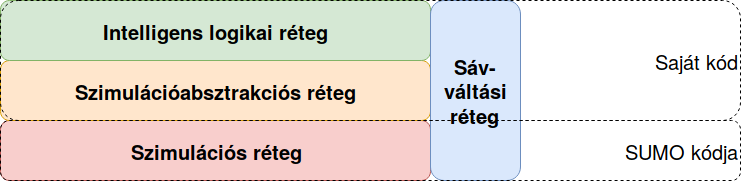
\includegraphics[width=1.0\textwidth]{retegmodell.png} 
			\caption{A rétegmodell szemléltetése}
			\label{pic:reteg}
		\end{figure}
		
	\section{Üzenetküldő rendszer}
		Korábban explicite szerepelt üzenetküldő rendszer a keretrendszer-implementációmban, most azonban úgy döntöttem, hogy az üzenetküldés függvényhívásokon keresztül meg. Univerzalitást pedig a közös, absztrakt alaposztály interfésze ad a rendszernek (pl. közlekedési csomópontok ősosztálya, járművek ősosztálya stb.). Erre főleg azért volt szükség, hogy a program áttekinthetőbb legyen, így ugyanis egy indirekcióval kevesebb szerepel a programkód szintjén.
		
		Ugyanakkor elméleti szinten továbbra is beszélek üzenetekről, ugyanis ez filozófiájában, leírásában igen szemléletes, csupán forráskód szintjén csak implicite jelenik meg.
		
	\section{Az intelligens keretrendszer alapfunkciói}
	\subsection{Csoportkezelés}
		\subsubsection{Markerrendszer}
			A csomópontok belépési pontjain belépési markerek vannak elhelyezve (lásd \aref{pic:szitu}.~ábrán). A belépési markerek jelzik a járművek számára, hogy be kell lépniük egy csoportba.
			
			A csomópontok kilépési pontjánál pedig kilépési markerek vannak, ezek jelzik, a csomópont elhagyását, a csportból való kilépés szükségességét.
			
			\begin{figure}[h]
				\centering
				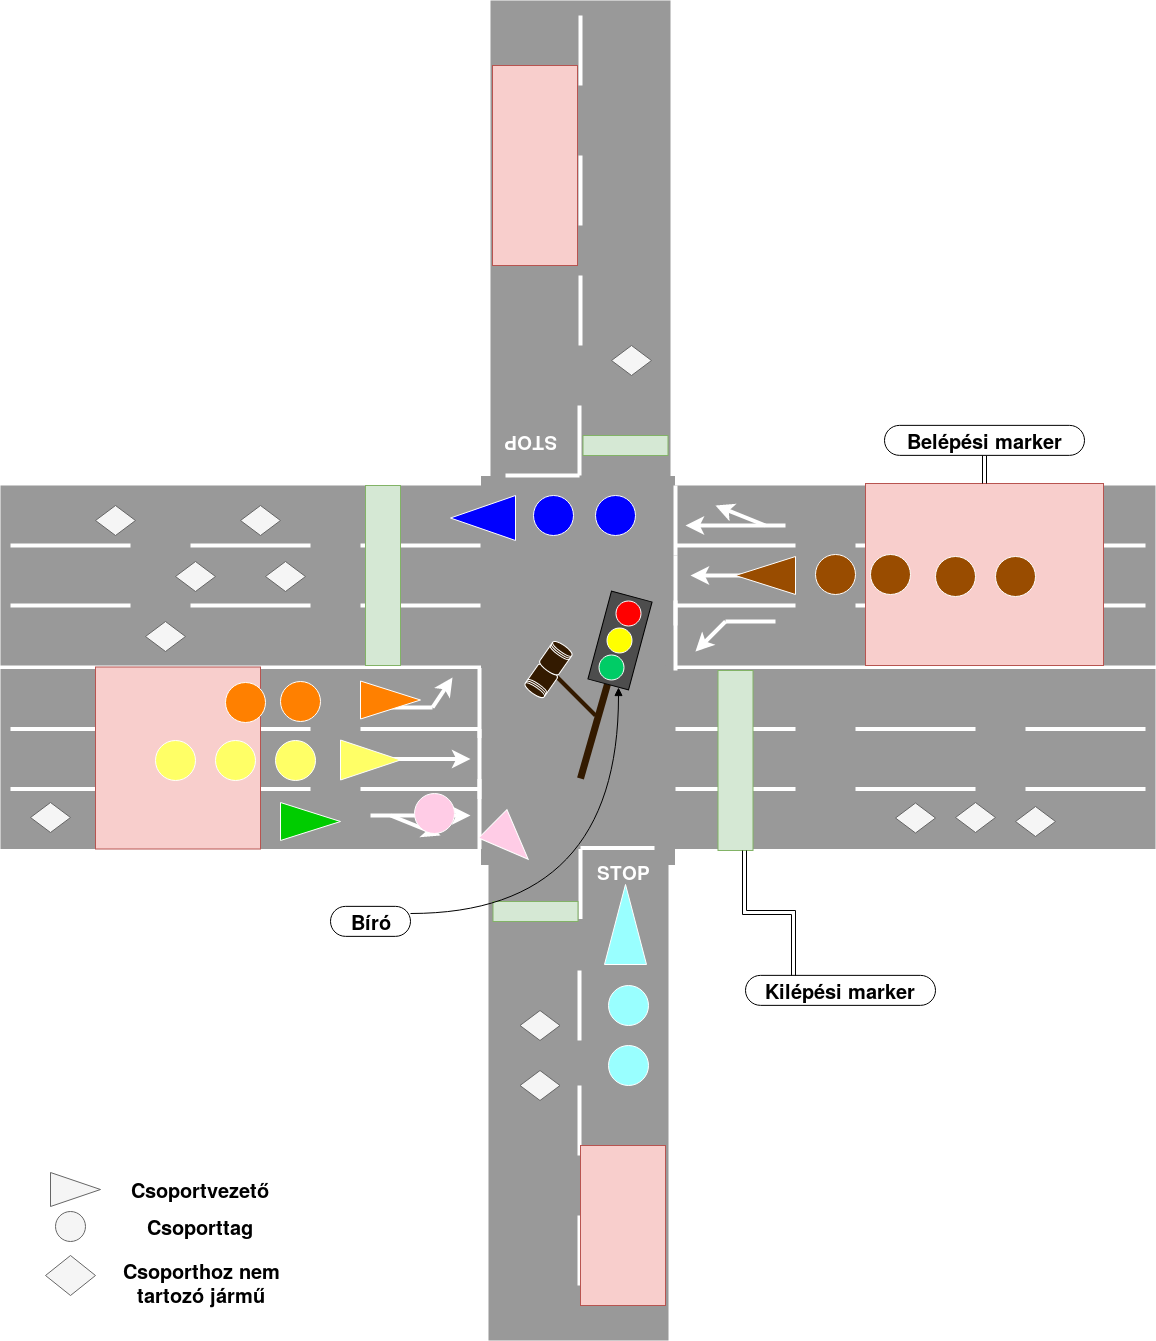
\includegraphics[width=1.0\textwidth]{szitu.png} 
				\caption{Példa a komponensekre}
				\label{pic:szitu}
			\end{figure}
			
		\subsubsection{Csoportformálás}
			Amikor a járművek egy csomópont közelébe érnek, akkor az egy pályán mozgó járművek (azok, amelyek egymás után jönnek egy sávban, és továbbhaladási irányuk megegyezik a csomópontban) csoportot formálnak. A csoportformálás akkor kezdődik, amikor egy autó a belépési markerre ér. A csoport elején haladó jármű a csoport vezetője, a csoport további tagjai őt követik. Amikor a csoportvezető a csomóponton történő áthaladás után a kilépési markerre ér, akkor kilép a csoportból, és a csoport vezetését a mögötte haladó csoporttagra adja át.
			
			Ez eltér a korábban alkalmazott módszertől. Az eltérést az indokolja, hogy így sokkal egyszerűbb egy csoport kettéosztását, egy preemptív csomóponti ütemezést megvalósítani.
			
			A megfelelő csoport kiválasztása belépési markerre érésnél a következő algoritmussal történik:
			\begin{enumerate}
				\item A jármű belépési markerre ér.
				\item A jármű megkérdezi, hogy az előtte haladó csoport (ha van ilyen) melyik kilépési pont felé halad.
				\item Ha megegyzik a haladási irány, akkor rákérdez arra, hogy csatlakozhat-e még a csoporthoz. Nem csatlakozhat akkor, ha a csoport aktuális mérete elérte megengedett legnagyobb csoportméretet.
				\item Ha a járművünk csatlakozhat a csoporthoz, akkor meg is teszi ezt, ellenkező esetben (vagy ha nincs előtte máisik jármű) pedig egy új csoportot alapít.
			\end{enumerate}
		
		\subsubsection{Viselkedési szabályok csoporton belül}
			A csoportot a csoportvezető irányítja. A csoportvezető dönt sávváltásokról. A csoporttagok követik a csoportvezetőt, illetve az előttük álló csoporttagokat. Csoporttagok nem előzhetik meg sem egy egymást, sem a csoportvezetőt.
			
			Ha a csoportvezető sávot váltott, akkor a csoporttagok a csoport elejétől kezdve egyesével sávot váltanak a csoportvezető által mutatott irányba.
			
			A csoporttagok egy P-szabályozó segítségével próbálnak meg egymástól megfelelő követési távolságot tartani. Ennek a szabályozónak a munkapontja jelenleg 10~m-re van beállítva.
			
			Természetesen jó lehetőség lenne a fogyasztás csökkentésére, ha minimalizálni tudnánk a követési távolságot, és a reakcióidőket kommunikációval javítanánk. Azonban ezzel a kérdéssel jelenleg nem foglalkozunk, ennek az előnyei amúgy is inkább egy gyorsforgalmi úton jelentkeznének főleg (nagyobb sebességénél nagyobb a szélárnyék, ami kedvezően hat a fogyasztásra).
			
	\subsection{Sávváltási rendszer}
		Az okos sávváltás alatt most a következő dolgot érthetjük. Csoportok haladnak párhuzamos közlekedésre alkalmas útszakaszon egymás mellett. Az egyik csoportnak \textit{(egónak)} sávot kell váltania azért, hogy a célja felé haladhasson tovább. Ekkor egy másik csoportot \textit{(altert)} megkér, hogy engedje be őt. Alter pedig lelassít vagy megáll, hogy ezt lehetővé tegye számára.
		
		A kommunikáció alter és egó csoportvezetője között zajlik, az egész csoportjukat ők képviselik. Alter teljesen altruistán viselkedik, amint egó kérést intéz felé, további mérlegelés nélkül végrehajtja egó kérését. Egó viszont megfontolja azt, hogy a beengedési kérése jogos-e alter felé.
		
		\subsubsection{Implementáció}
			Kiindulási alapként a SUMO kódbázisával érkező ``SL2015''-ös névre hallgató alsávmodellt is tartalmazó osztályát használtam. Ez az alapkód már tartalmaz logikát annak eldöntésére, hogy éppen sávot kell-e váltani. Abban az esetben, ha igen, azt is meghatározza, hogy a célsávon haladó gépjármű elé vagy mögé érdemes-e váltani, majd ezt a szomszédos járművel le is kommunikálja.
			
			Ehhez a számításhoz saját paraméterei közül csak a járműhosszát használja. Ezt kis módosítással a csoport hosszára változtattam, majd teszteltem, hogy ez milyen befolyással van a program működésére. Bebizonyosodott, hogy alapvetően az elvárásoknak megfelelő hatása van.
			
			Mivel alter -- ahogy már szó volt róla -- altruista viselkedésű, ezért némiképp módosítani kellett a beengedő algoritmust is, hogy elérjük ezt az önfeláldozó viselkedést.
			
			
	\subsection{Csomóponti rendszer}
		A csomópontok vagy bírók felelősek azért, hogy a közlekedési csomópontokon az összes jármű biztonságban, és lehetőleg minél gyorsabban átjuthasson. Keretrendszeri szinten ez egy teljesen absztrakt konstrukció, a megvalósítása már a keretrendszertől független, ugyanis kellően messze van már a szimulációs rétegtől. Egy példát láthatunk \aref{pic:abs}.~ábrán, ahol az AbstractJudge és ConflictClass a keretrendszer által adott osztályok, míg ezek leszármazottjai azok egy-egy konkrét implementációja.
		
		\begin{figure}[h]
			\centering
			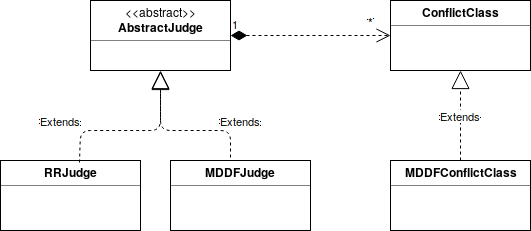
\includegraphics[width=1.0\textwidth]{absztrbiro.png} 
			\caption{Az absztrakt osztályok szemléltetése}
			\label{pic:abs}
		\end{figure}
		
		\subsubsection{Konfliktusosztályok}
			Azon autócsoportok, akik egyszerre áthaladhatnak a közlekedési csomóponton, azok egy konfliktusosztályt alkothatnak. Azon autók haladhatnak át egyszerre egy közlekedési csomóponton, akik egymást nem metsző pályán mozognak.
			
			A konfliktusosztályba sorolás implementációfüggő, a keretrendszer a konkrét megvalósítástól független, bár egy alapvető implementációt kényelmi okokból nyújt.
			
		\subsubsection{A bíró, mint ütemező}
			A bíró feladata, hogy a konfliktusosztályok közül kijelölje, hogy ki haladhat át a csomóponton. A konkrét megvalósítás itt is implementációfüggő, de alapvetően az operációs rendszerek ütemezői szolgáltatják az algoritmusok ötletét.
			
		\subsubsection{Preempció és megvalósítása}
			Mint az operációs rendszerek ütemezői, a bírólogika is viselkedhet preemptív módon, azaz megszakíthatja bizonyos konfliktusosztályok áthaladását, még akkor is, ha a konfliktusosztályt képző járműcsoportok még nem teljes egészében haladtak is át.
			
			Hogy ez létre jöhessen, az egyes járműveket külön-külön kezeljük, nem csoportszinten. Az egyes járművek pollingozással, periodikusan lekérdezik a bírót, hogy áthaladhatnak-e a csomóponton. Amennyiben a válasz nemleges, és még nem haladtak át egy olyan ponton, ahol már nem lehet biztonsággal megállni, a járművek lelassítanak, szükség esetén megállnak (jelenleg a csomópont közepétől 25~m-re).
			
			Ez azért hatékony megoldás, mert egy csoportvezető pl. áthaladhat még a csomóponton, a rögtön őt követő csoporttag meg már nem. Ebben az esetben a csoporttag megáll, a csoportvezető pedig eléri a kilépési markert, és ezzel a csoport vezetését már rá is bízta az immár álló csoporttagra.
			
	\section{Néhány gyakorlati példa}
		\subsection{Bíróimplementációk}
			\subsubsection{Round Robin alapú bíró}
				A keretrendszer kipróbálásaként implementáltam egy Round Robin jellegű csomóponti logikát. Ez gyakorlatilag egy klasszikus rendőrlámpa ``intelligens'' megfelelője.
				
			\subsubsection{MDDF alapú ütemező}
				Operációs rendszerek témaköréből ismerjük, hogy a legrövidebbet előre elnevezésű (Shortest Job First, SJF) ütemező optimális az átlagos várakozási időkre nézve. A forgalomszimulációban az algoritumus löketidőbecsléseként a célig hátralévő távolságot vesszük, ahogyan azt \acite{MDDF}-ben olvashatjuk.
				
				Tehát ez az implementáció a következőképpen működik:
				\begin{enumerate}
					\item A mozgáspályáknak megfelelően konfliktusosztályokba soroljuk a járműcsoportokat.
					\item Bizonyos időközönként (pl. 3 másodpercenként) meghatározzuk, hogy melyik konfliktusosztályban van az a jármű, amely a legközelebb van a célállomásához.
					\item Az előző lépésben megtalált konfliktusosztályt jelöljük következő áthaladónak.
				\end{enumerate}
			
				Jelenleg ennek az implementációja még nincsen sajnos kész.
				
		\subsection{Jövőbeli felhasználási lehetőségek}
			\subsubsection{Megkülönböztető jelzést használó járművek kezelése}
				A keretrendszer segítségével lehetőség nyílna megvizsgálni, hogyan lehet javítani a megkülönböztető jelzést használó járművek előrehaladását egy sűrű városi forgalomban.
				
				Ez egy igen fontos kérdés, hiszen a jelenlegi közlekedés egyik nagyon sarkalatos pontja az, hogy a járművezetők hogyan reagálnak, ha egy szirénázó mentő, rendőr, tűzoltó megjelenik az úton. Sajnos a mindennapi tapasztalatunk azt mutatja, hogy ritkán sikerül igazán segíteni az előrejutásukat. Éppen ezért lenne előnyös kidolgozni eljárásokat, módszereket arra, hogy egy intelligens rendszer hathatósan segítse a megkülönböztető jelzést használó járművek haladását.
				
				Itt érdekes kérdés, hogy a rendszer hogyan tudja előre engedni a szirénázó gépjárműveket. Vagy egy intelligens közlekedési csomópont hogyan tudja biztosítani a mielőbbi áthaladását úgy, hogy közben a forgalom többi résztvevője is biztonságban marad.
				
			\subsubsection{MI-beli algoritmusok használata forgalomirányításra}
				Az absztrakt bírólogika megengedi, hogy bármilyen forgalomirányító algoritmust implementálhassunk. Érdekes kérdés lehet, hogyha nem egy klasszikus megközelítést (Round Robin vagy valamilyen operációs rendszerütemezőt) használunk, hanem valamilyen mesterséges intelligenciából ismert algoritmusra (pl. A*) építünk.
				
				Érdekes lehet, hogy nyerünk-e ezzel valamit a klasszikus rendőrlámpás vagy egy MDDF-alapú megoldáshoz képest. Ugyancsak érdekes, hogy mi történik akkor, ha egy ilyen rendszerben egy megkülönböztető jelzést használó gépjármű szeretne áthaladni a csomóponton.
				
	\begin{thebibliography}{9}
		\bibitem{sumo} D. Krajzewicz, J. Erdmann, M. Behrisch, és L. Bieker, ``Recent Development and Applications of SUMO – Simulation of Urban MObility'', o. 11, 2012.
		
		\bibitem{MDDF} F. Ahmad, S. A. Mahmud, G. M. Khan, és F. Z. Yousaf, ``Shortest remaining processing time based schedulers for reduction of traffic congestion'', in 2013 International Conference on Connected Vehicles and Expo (ICCVE), Las Vegas, NV, USA, 2013, o. 271–276.
		
	\end{thebibliography}
\end{document}